\documentclass[aspectratio=169]{beamer}
\usepackage[utf8]{inputenc}
\usepackage{graphicx}
\usepackage{hyperref}
\usepackage{multicol}

% Add search paths for images (slides + CERN theme assets)
\graphicspath{{screenshots/}{../screenshots/}{presentation_latex/cern-beamer/}{presentation_latex/cern-beamer/logos/}{cern-beamer/}{cern-beamer/logos/}}

% CERN Beamer theme
\usetheme{CERN}
\setbeamerfont{frametitle}{size=\large}
\setbeamerfont{normal text}{size=\small}
\setbeamerfont{itemize/enumerate body}{size=\small}
\setbeamerfont{itemize/enumerate subbody}{size=\small}

% Date shown in footer and title page
\def\mydate{15 Feb 2025}

% Title metadata
\title{A GUI for Magboltz}
\subtitle{IFIN-HH (Romania)\\7th DRD1 Collaboration Meeting\\WG4 --- Modeling and Simulations}
\author{Michele Renda\\\texttt{michele.renda@cern.ch}\\Dan Andrei Ciubotaru\\\texttt{andrei.ciubotaru@cern.ch}}

\begin{document}

% Slide 1 — Title
\begin{frame}
  \titlepage
\end{frame}

% Slide 2 — Context & Workflow
\begin{frame}{Magboltz: Context \& Workflow}
\begin{columns}[T]
  \column{0.5\textwidth}
    \textbf{Why it matters}
    \begin{itemize}
      \item Monte Carlo electron transport simulation
      \item Fundamental tool for detector physics
      \item Used across MPGDs, TPCs, RPC studies
    \end{itemize}
  \column{0.5\textwidth}
    \textbf{CLI friction}
    \begin{itemize}
      \item Text-based input cards
      \item Manual output parsing
      \item Iterative tuning \& plotting scripts
      \item Student onboarding difficulty
    \end{itemize}
\end{columns}
\vspace{0.2cm}
\textbf{Cornerstone physics engine, workflow-heavy interface.}
\end{frame}

% Slide 3 — Workflow Pipeline
\begin{frame}{Workflow Pipeline}
\vspace{0.2cm}
\begin{center}
\Large
Input \(\rightarrow\) Run \(\rightarrow\) Parse \(\rightarrow\) Export \(\rightarrow\) Plot
\end{center}
\vspace{0.4cm}
\begin{center}
\textbf{We change the workflow, not the physics.}
\end{center}
\end{frame}

% Slide 4 — Introducing Magboltz GUI
\begin{frame}{Magboltz GUI}
\begin{columns}[T]
  \column{0.48\textwidth}
    \begin{itemize}
      \item Python + PyQt6 application
      \item Cross-platform
      \item Designed as a workflow layer, not a replacement
      \item Core functions:
        \begin{itemize}
          \item Input file creation \& editing
          \item Gas mixture editor \& visual pie chart
          \item Magboltz execution wrapper
          \item Output parsing $\rightarrow$ structured model
          \item Data export $\rightarrow$ CSV / JSON / XML
          \item Built-in plotting tools
        \end{itemize}
    \end{itemize}
  \column{0.52\textwidth}
    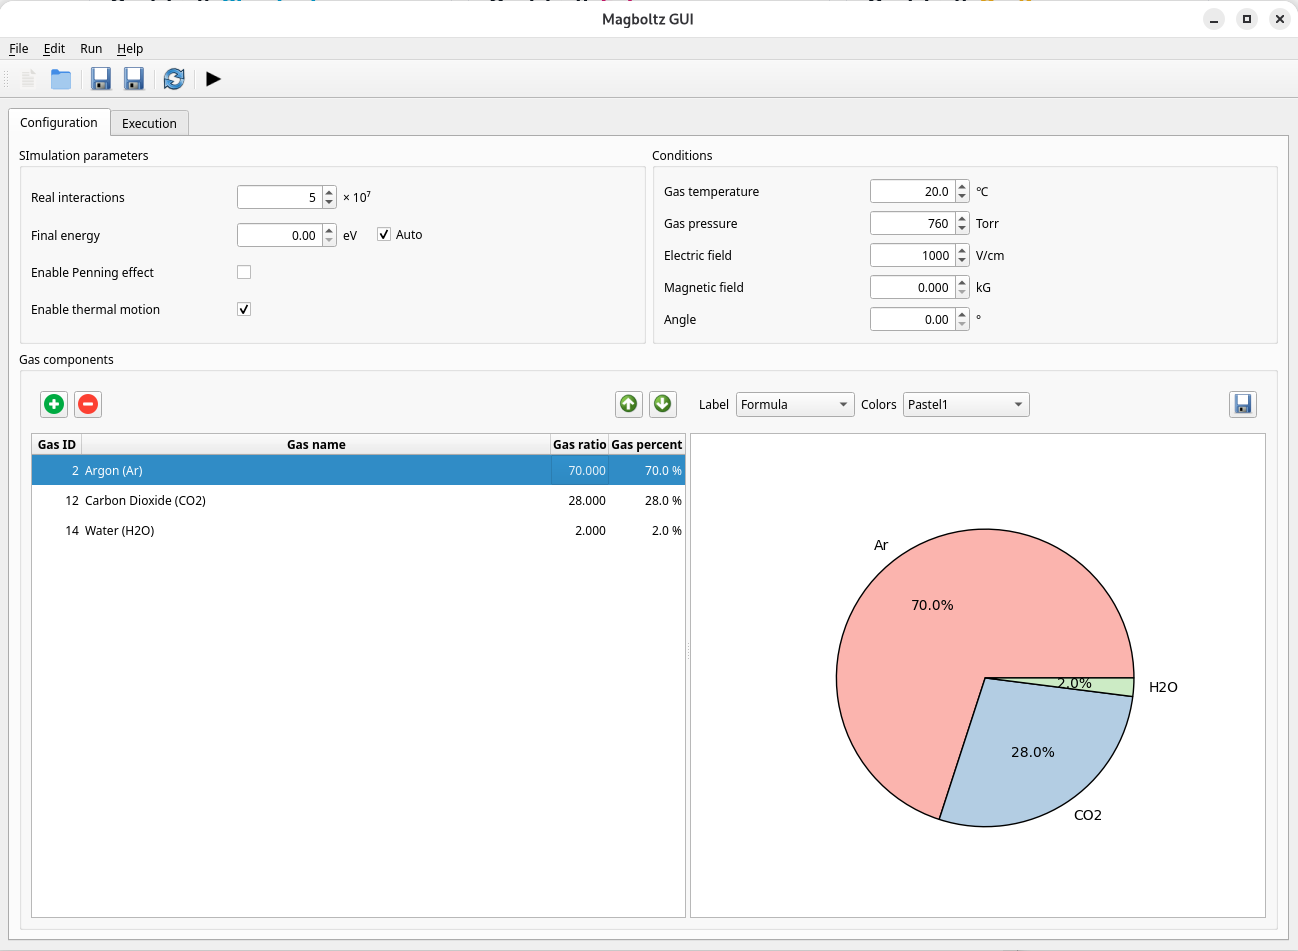
\includegraphics[width=\textwidth]{main_window.png}
\end{columns}
\end{frame}
% Slide 5 — Execution & Output Handling
\begin{frame}{Execution Workflow}
\begin{columns}[T]
  \column{0.48\textwidth}
    \begin{itemize}
      \item Direct Magboltz invocation
      \item Command line transparency
      \item Live stdout/stderr streaming
      \item Run/Stop controls
      \item Raw output persistence
      \item Reopen previous runs
    \end{itemize}
  \column{0.52\textwidth}
    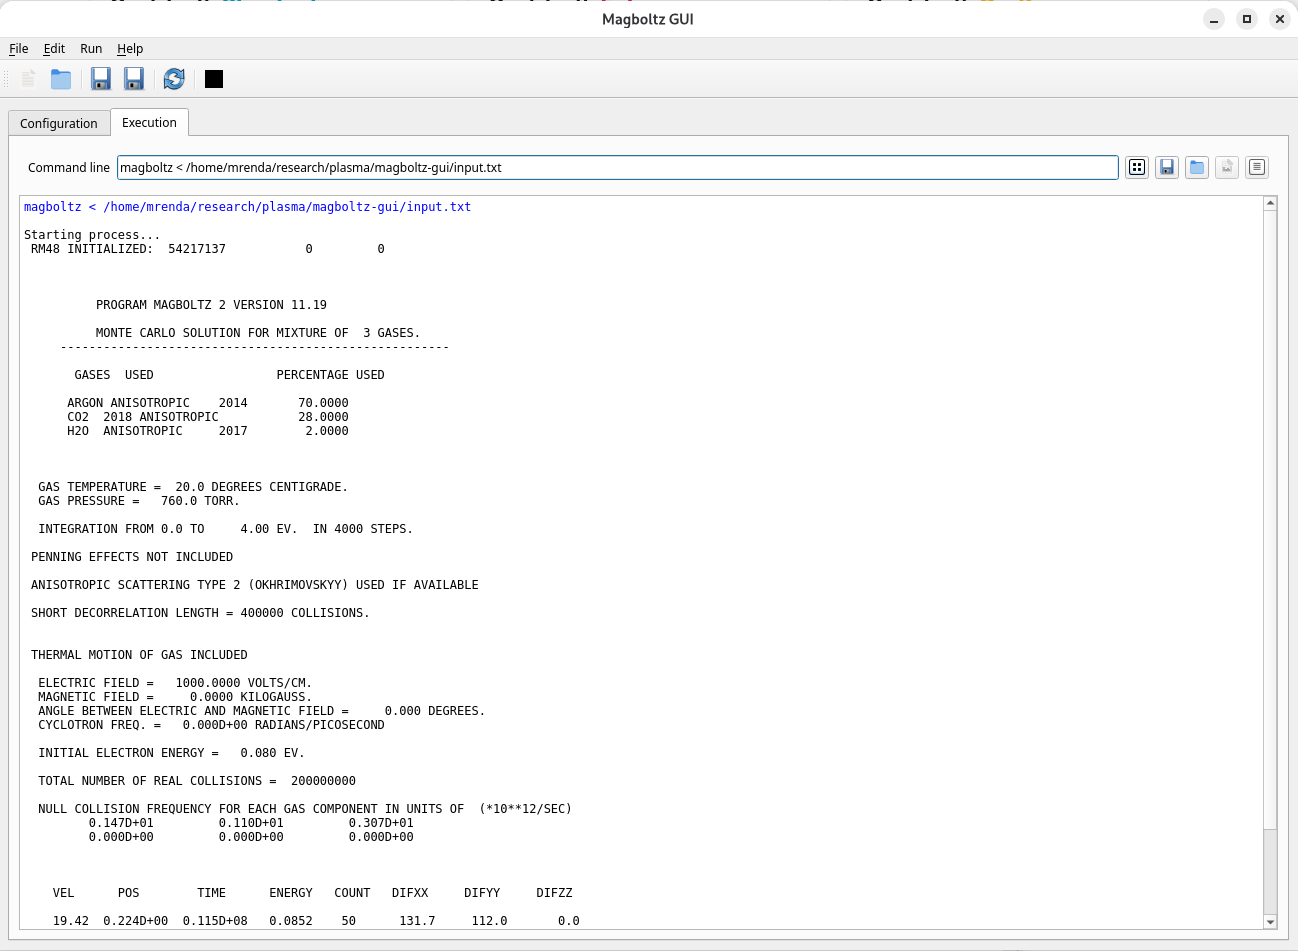
\includegraphics[width=\textwidth]{execution_tab_running_output.png}
\end{columns}
\end{frame}

% Slide 6 — What This Does NOT Do
\begin{frame}{What This Does NOT Do}
\begin{itemize}
  \item Does \textbf{not} change Magboltz physics, models, or algorithms
  \item Does \textbf{not} alter input semantics or units
  \item Does \textbf{not} replace the CLI (it wraps it)
  \item Does \textbf{not} ship the Magboltz binary
\end{itemize}
\end{frame}

% Slide 7 — Validation \& Trust
\begin{frame}{Validation \& Trust}
\begin{itemize}
  \item Parsed outputs are \textbf{1:1} with Magboltz text output
  \item No unit conversions; values are preserved as printed
  \item Export schema is versioned (\texttt{v1.0})
  \item Raw output \& parser warnings are retained
\end{itemize}
\end{frame}

% Slide 8 — Structured Parsing & Exports
\begin{frame}{From Text Output $\rightarrow$ Structured Data}
\begin{columns}[T]
  \column{0.48\textwidth}
    \begin{itemize}
      \item Canonical RunResult model
      \item Extracted:
        \begin{itemize}
          \item Transport coefficients
          \item Collision frequencies
          \item Convergence tables
          \item Energy distributions
        \end{itemize}
      \item Export formats:
        \begin{itemize}
          \item CSV
          \item JSON
          \item XML
        \end{itemize}
      \item Reproducible analysis pipelines
    \end{itemize}
  \column{0.52\textwidth}
    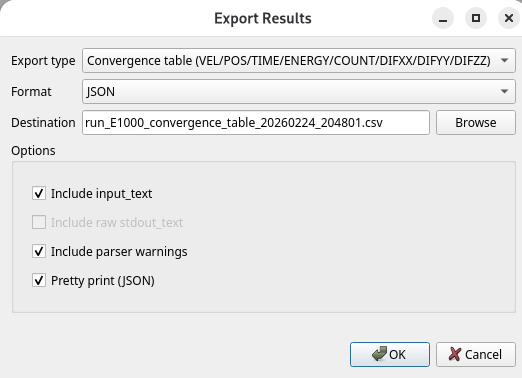
\includegraphics[width=\textwidth]{export_window.png}
\end{columns}
\end{frame}

% Slide 9 — Plotting & Rapid Exploration (1/2)
\begin{frame}{Built-in Plotting Tools}
\vspace{-0.2cm}
\begin{center}
\begin{tabular}{cc}
  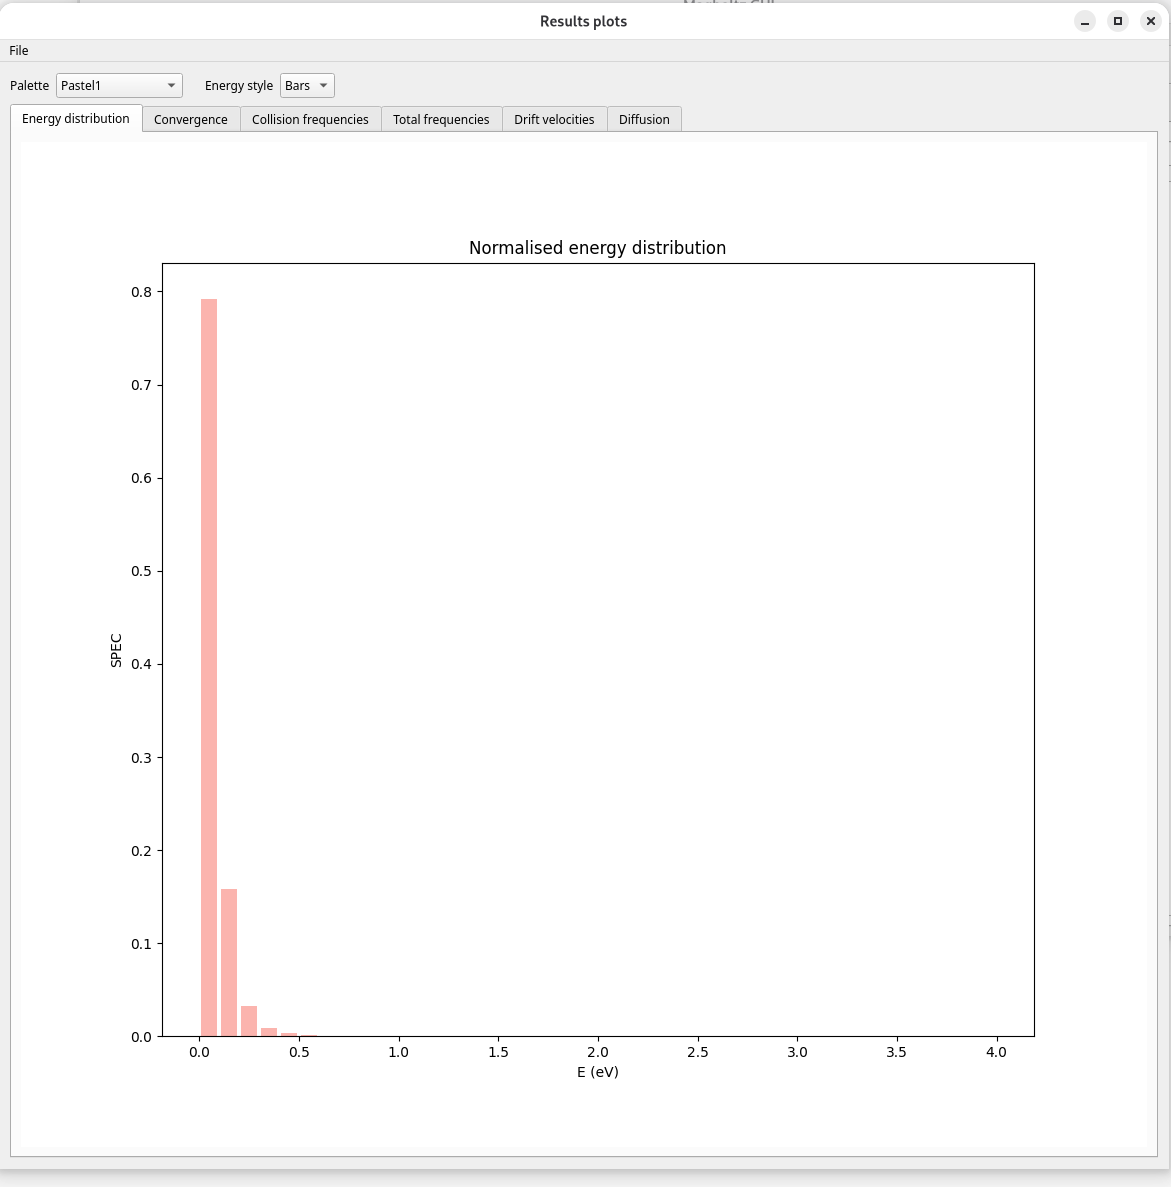
\includegraphics[width=0.48\textwidth,height=0.55\textheight,keepaspectratio]{plots_energy_distribution_bars.png} &
  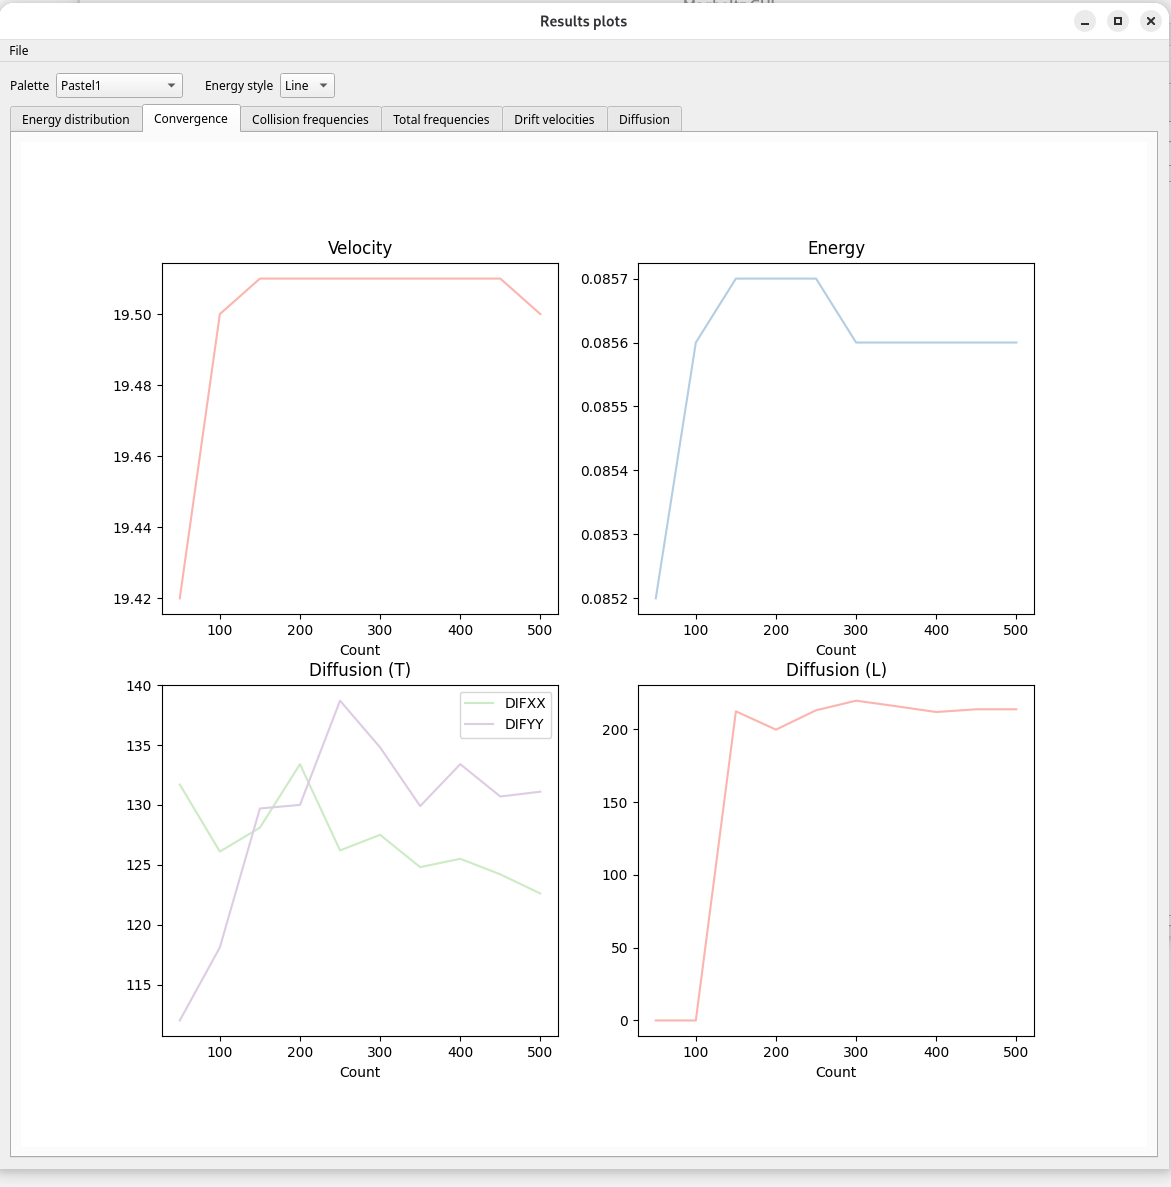
\includegraphics[width=0.48\textwidth,height=0.55\textheight,keepaspectratio]{plots_convergence.png} \\
  \scriptsize Energy distribution & \scriptsize Convergence
\end{tabular}
\end{center}
\vspace{-0.05cm}
\textbf{Immediate visual feedback without external scripts.}
\end{frame}

% Slide 10 — Plotting & Rapid Exploration (2/2)
\begin{frame}{Built-in Plotting Tools (cont.)}
\vspace{-0.2cm}
\begin{center}
\begin{tabular}{cc}
  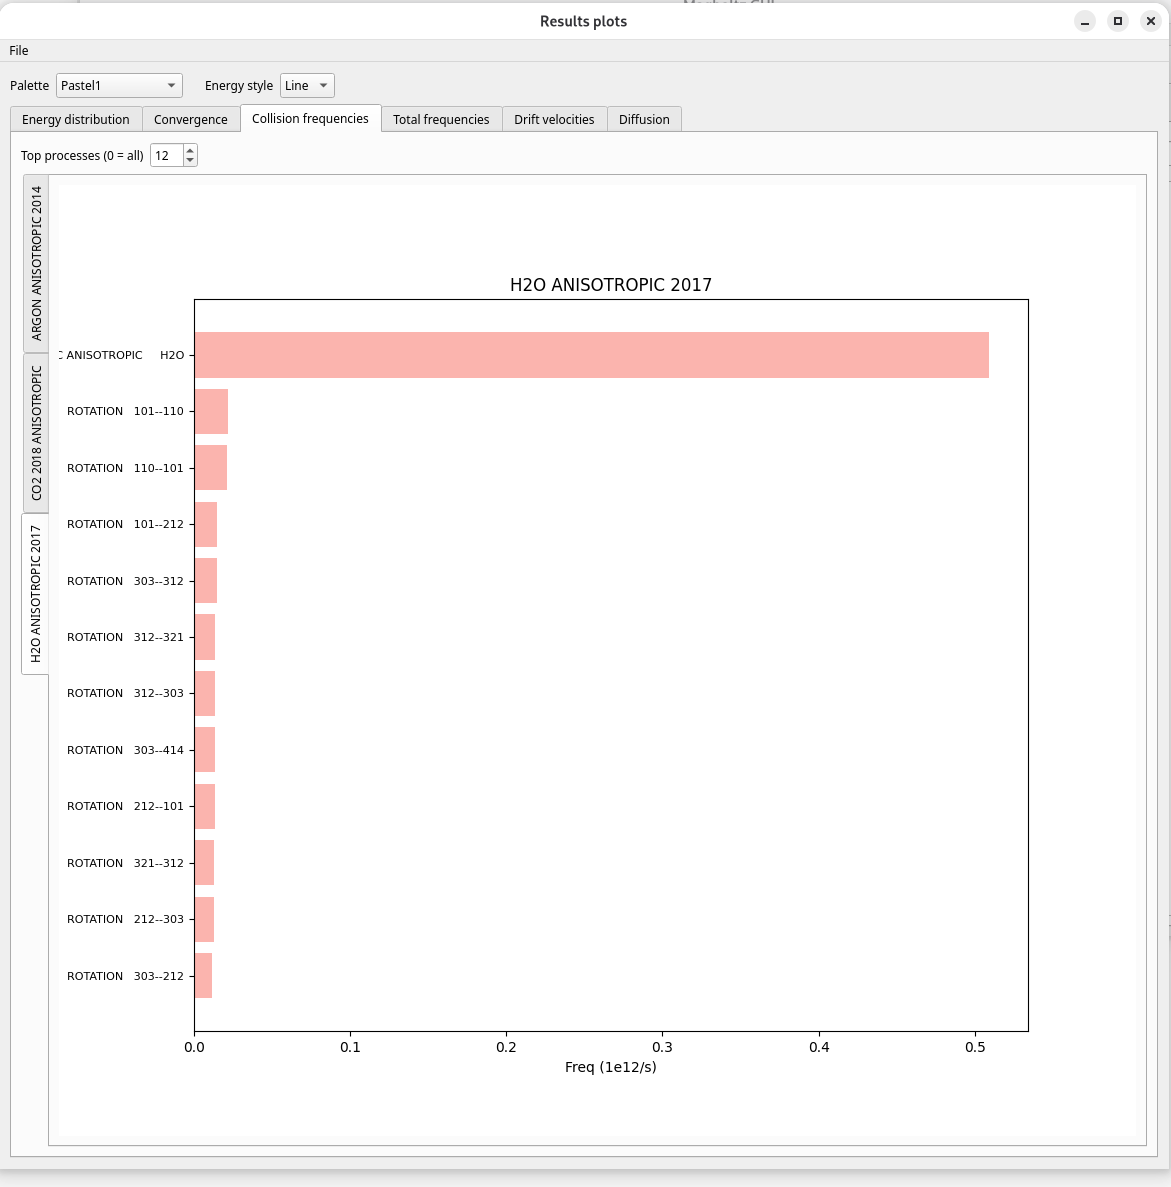
\includegraphics[width=0.48\textwidth,height=0.55\textheight,keepaspectratio]{plots_collision_frequencies.png} &
  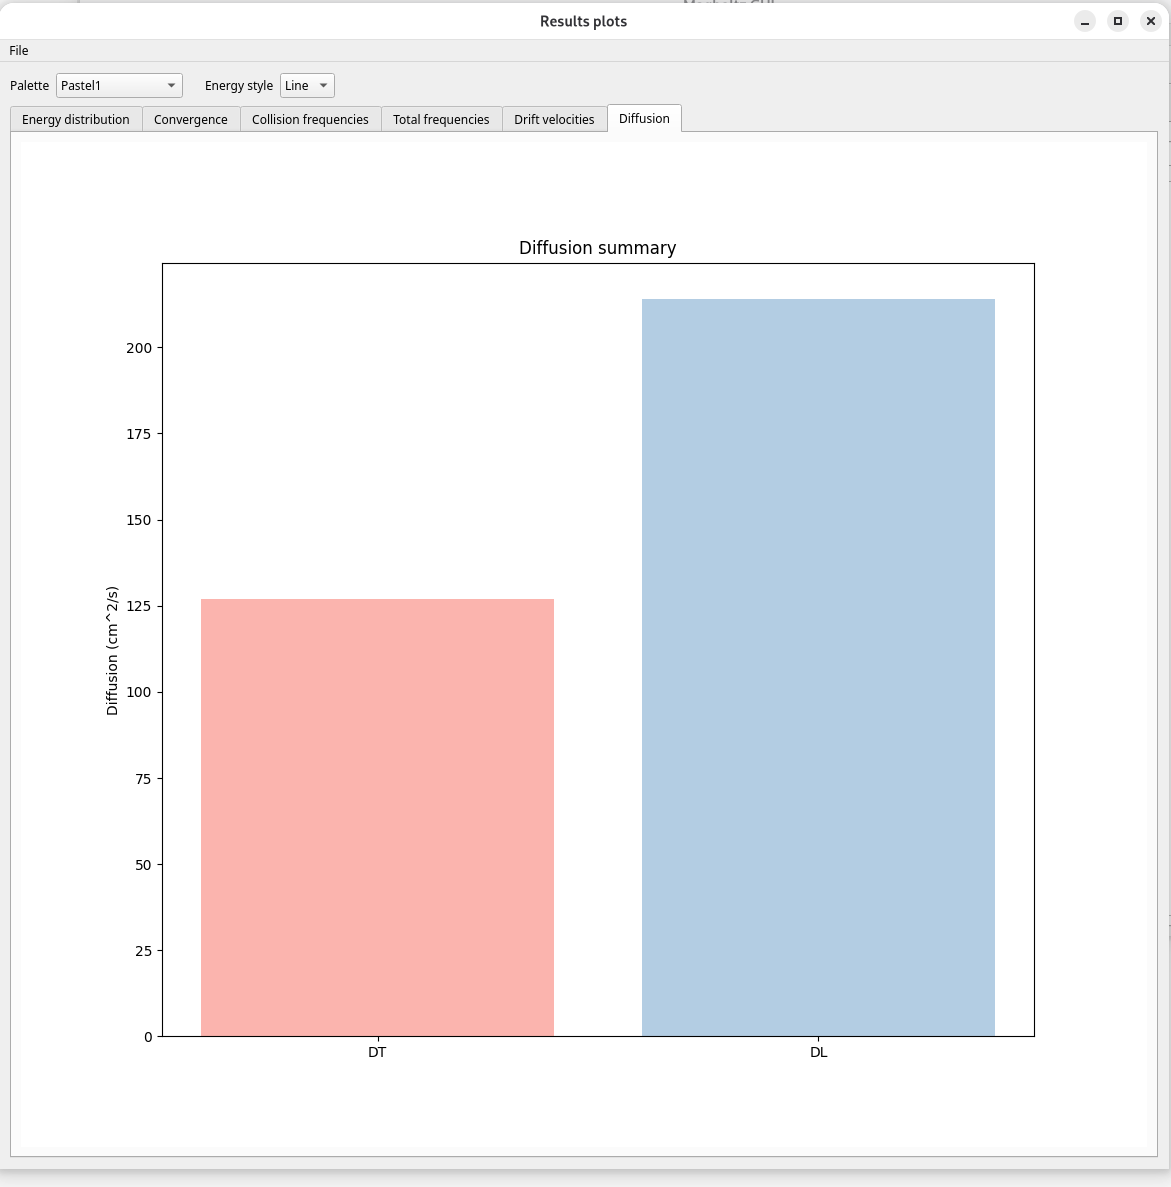
\includegraphics[width=0.48\textwidth,height=0.55\textheight,keepaspectratio]{plots_diffusion_summary.png} \\
  \scriptsize Collision frequencies & \scriptsize Diffusion summary
\end{tabular}
\end{center}
\vspace{-0.05cm}
\textbf{Immediate visual feedback without external scripts.}
\end{frame}

% Slide 11 — Availability & License
\begin{frame}{Availability \& License}
\textbf{Project repository}
\vspace{0.2cm}

\begin{itemize}
  \item GitLab: \texttt{https://gitlab.com/micrenda/magboltz-gui/}
  \item License: MIT
  \item Documentation: README in the repository
\end{itemize}
\end{frame}

% Slide 12 — Setup (pip + bundled Qt)
\begin{frame}[fragile]{Setup: pip (bundled Qt)}
\textbf{Recommended when you want Qt bundled with the app.}
\vspace{0.3cm}

\begin{itemize}
  \item Python environment
  \item Magboltz binary available in PATH
\end{itemize}

\textbf{Commands:}
\begin{verbatim}
pip install "magboltz-gui[qt]"
magboltz-gui
\end{verbatim}
\end{frame}

% Slide 13 — Setup (pip + system Qt)
\begin{frame}[fragile]{Setup: pip (system Qt)}
\textbf{Recommended on Linux when using system PyQt6.}
\vspace{0.3cm}

\begin{itemize}
  \item Install system Qt bindings
  \item Magboltz binary available in PATH
\end{itemize}

\textbf{Commands (Debian/Ubuntu):}
\begin{verbatim}
sudo apt install python3-pyqt6
pip install magboltz-gui
magboltz-gui
\end{verbatim}
\end{frame}

% Slide 14 — Limitations & Next Steps
\begin{frame}{Limitations \& Next Steps}
\begin{itemize}
  \item No batch sweeps yet; single-run workflow
  \item Limited automation for parameter scans
  \item Next: parameter scan runner + input templates
  \item Next: headless export-only mode for pipelines
\end{itemize}
\end{frame}

% Slide 15 — Tribute
\begin{frame}{In Memoriam}
\vspace{0.3cm}
\begin{center}
\large
\textbf{Stephen F. Biagi}\\
{\footnotesize (1949--2025)}\\
\vspace{0.25cm}
We dedicate this work to his memory.\\
\vspace{0.25cm}
His pioneering contributions to modeling\\
electron transport in gases profoundly shaped\\
detector physics.\\
\vspace{0.35cm}
\normalsize
This interface is a modest tribute to his legacy.
\end{center}
\end{frame}

\end{document}
